\section*{Hierarchical clustering}

Hierarchical clustering contains two types of methods:

- Agglomerative: bottom-up approach (from leaves to root)

- Divisive: top-to-bottom (from root to leaves)\\

\underline{Agglomerative clustering} \\

Agglomerative clustering is a sequential process:

- First, all data points are considered as separate clusters.

- Then, step by step, clusters that are closed to each other merge. \\

The first two steps of an example are displayed below:

\begin{center}
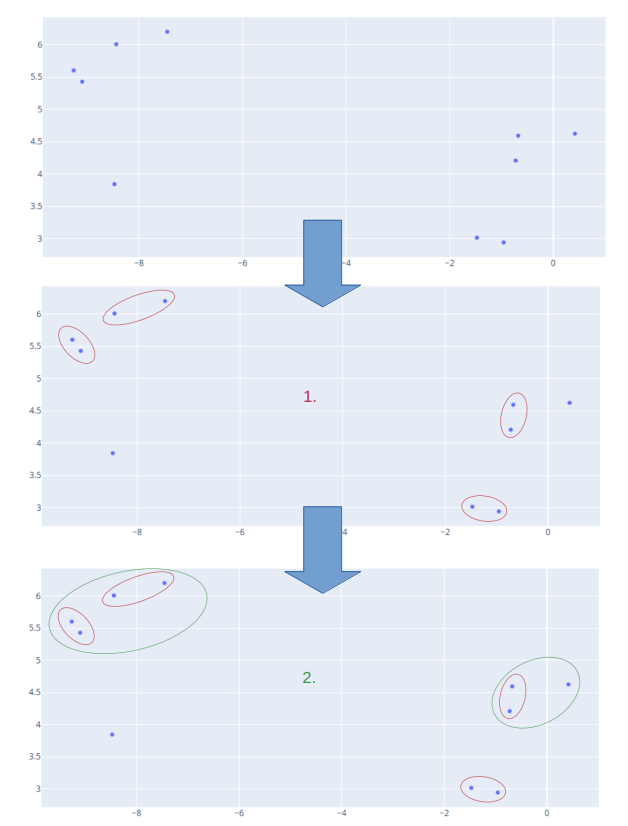
\includegraphics[scale=0.4]{hierarchical_clustering_steps.png}
\end{center}

The whole merging process can be vizualized using a dendrogram where the y-axis is the distance between two points/clusters. In x-axis we see the data point index.

\begin{center}
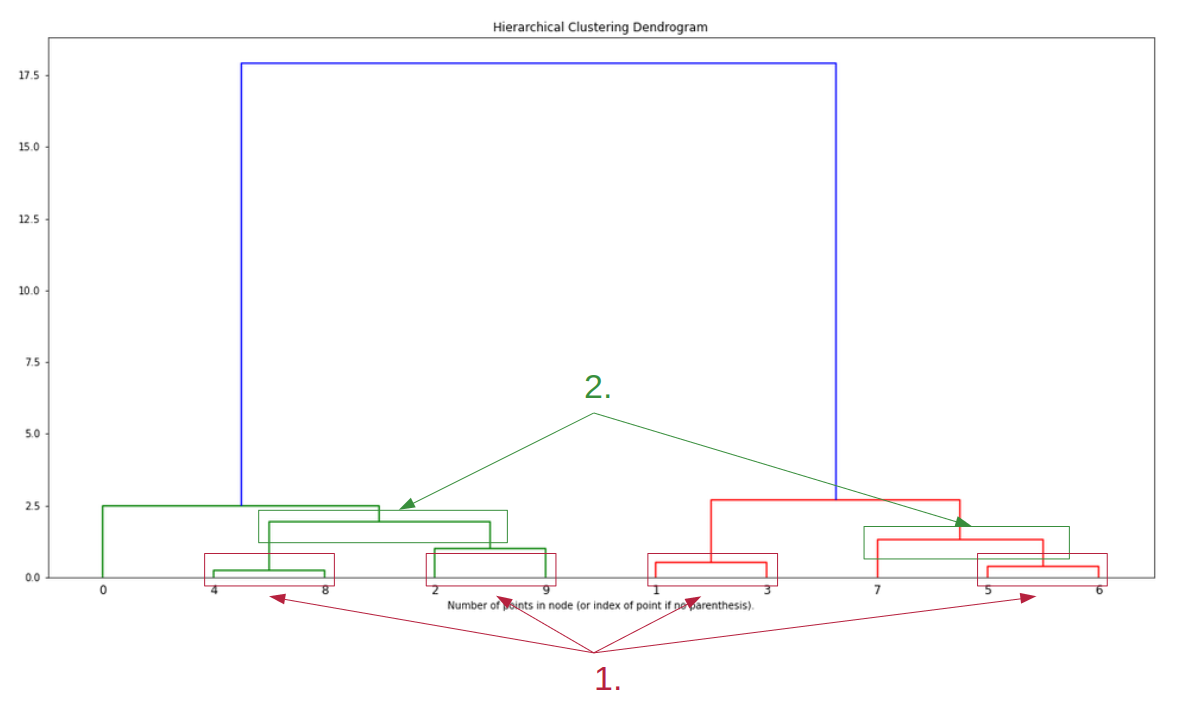
\includegraphics[scale=0.4]{agg_clustering_dendrogram.png}
\end{center}

\textit{Note}:  In case of a large sample, it is possible to display only the last steps of the algorithms (see \textit{level} parameter in scipy). \\

There are three main parameters to choose:

- Distance metric: this is the metric used to compute the distance between two \textbf{data points}.

- Distance function / rules: this is the function used to compute distance between two \textbf{clusters}. It's a function of the distance metric.

- Number of clusters \\

\textit{Distance functions} \\

The most common distance functions are: \\

Minimum distance (also called \textit{single-linkage-clustering}):

$$D(A,B) = min\{d(x,y): x \in A, y \in B\}$$

Average distance:

$$D(A,B) = \frac{1}{|A| |B|} \sum_{x \in A,~y \in B}d(x,y)$$

Max distance (also called \textit{complete-linkage-clustering}):

$$D(A,B) = max\{d(x,y): x \in A, y \in B\}$$ \\

\begin{center}
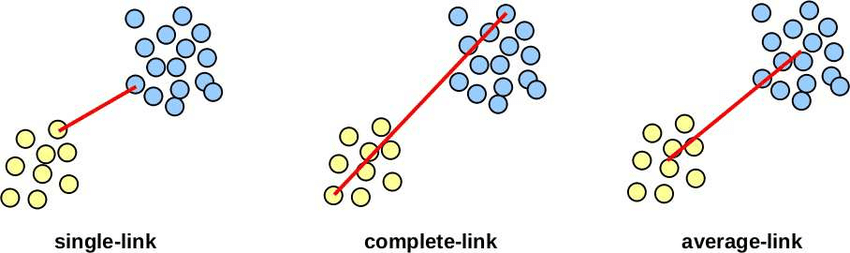
\includegraphics[scale=0.5]{linkage-distance.png}
\end{center}

\textit{Number of clusters} \\

To select the number of clusters, we can look at the dendrogram: we focus on groups that are linked by long lines. Since the lines represent the distance between data points or clusters, a group of clusters that are far away from each other will be linked with long lines.

In the below dendogram, it's quite clear that 3 clusters are well separated:

\begin{center}
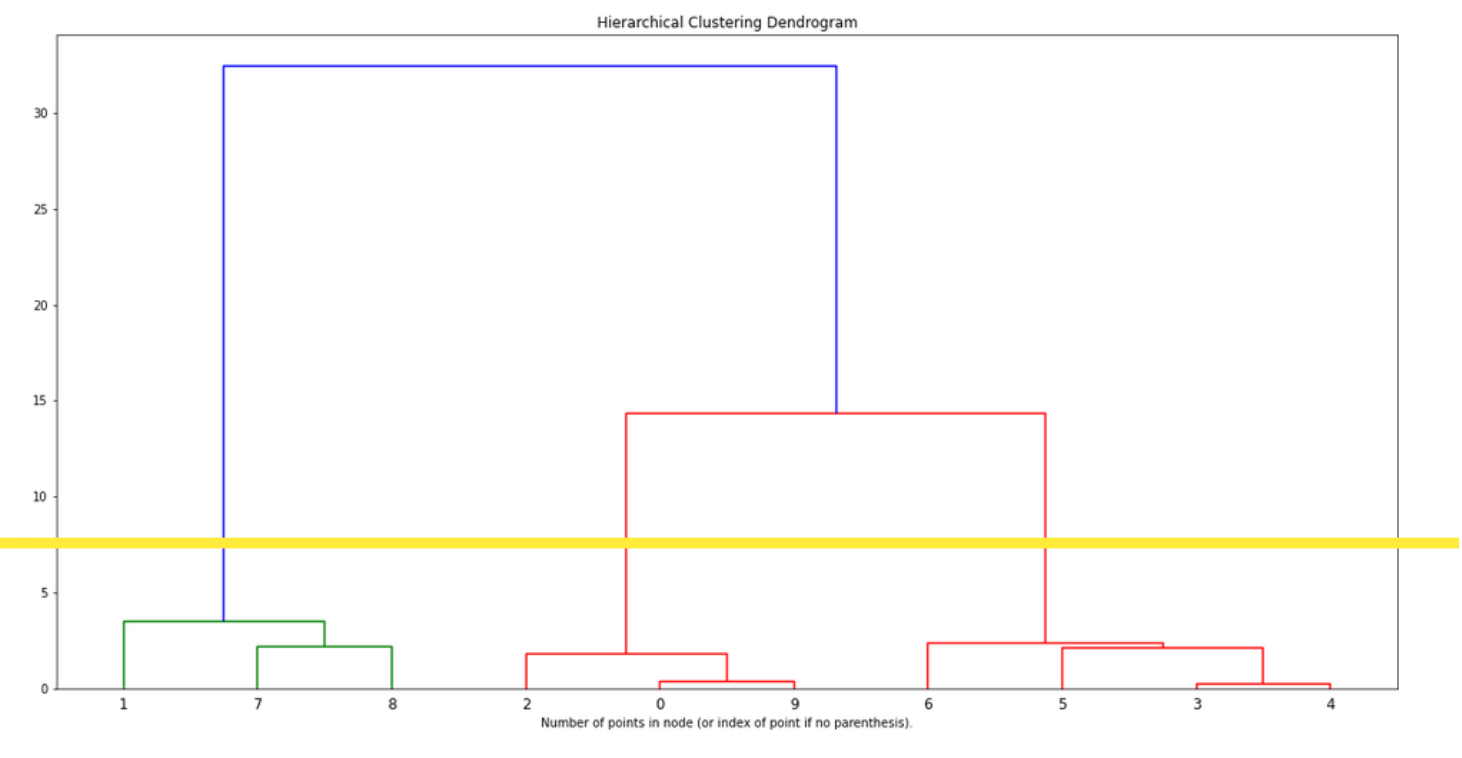
\includegraphics[scale=0.3]{clustering_3.png}
\end{center}

On the below example (with associated dataset), we could select 3 or 5 clusters.

\begin{center}
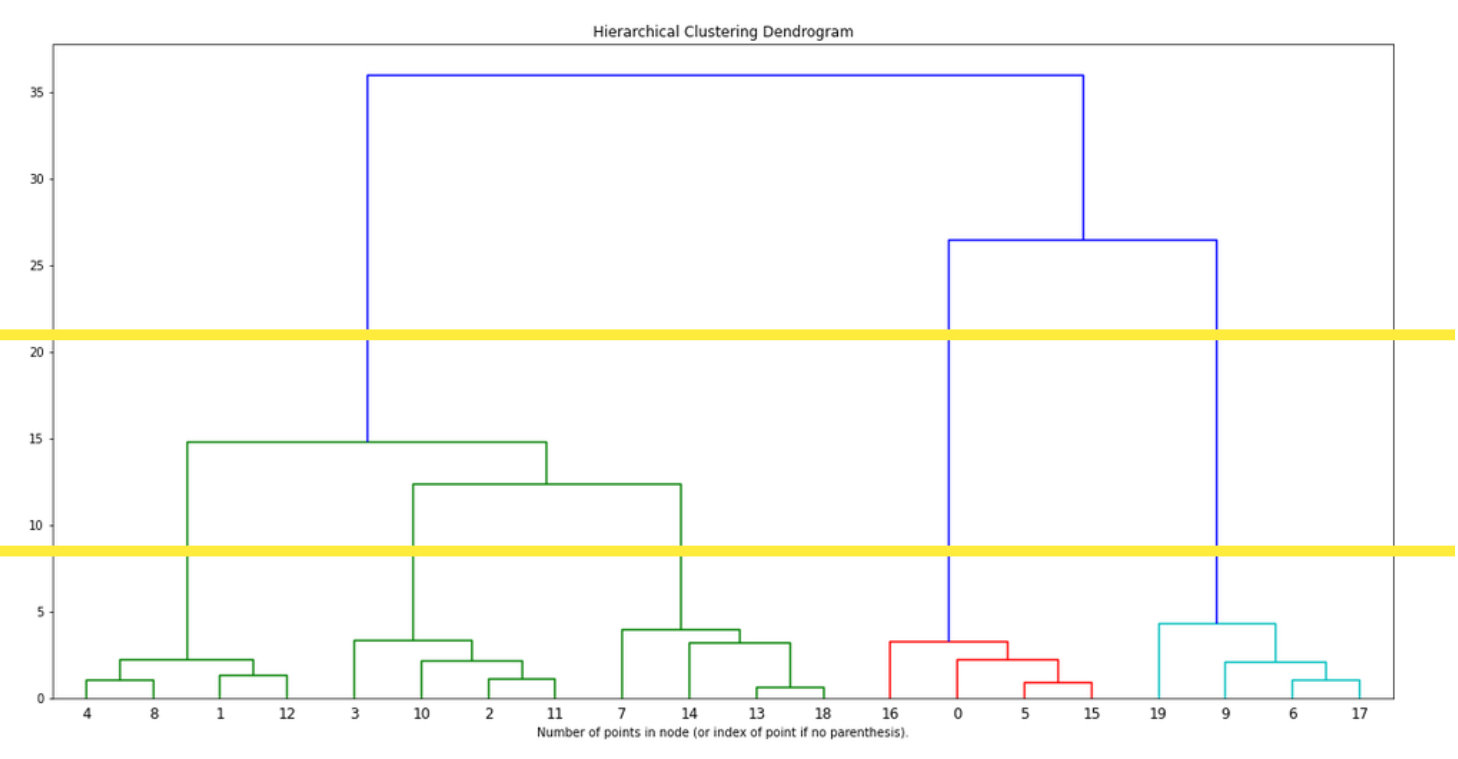
\includegraphics[scale=0.3]{clustering_5.png}
\end{center}

\begin{center}
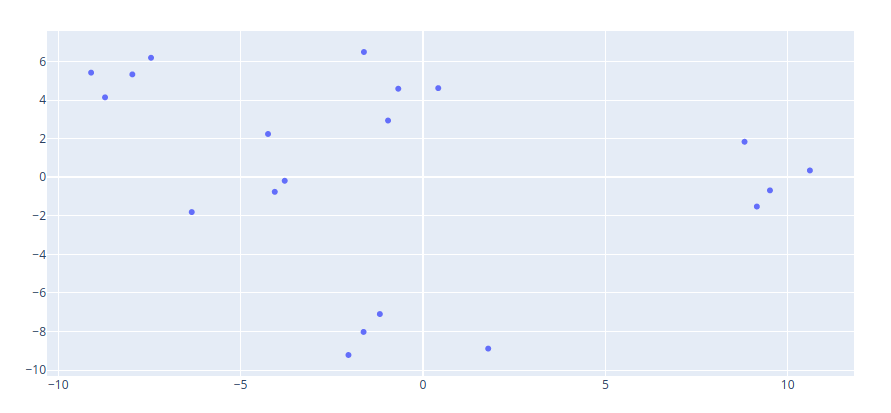
\includegraphics[scale=0.4]{clustering_5_data.png}
\end{center}





